\documentclass{ximera}
\graphicspath{     %% setup a global graphics path
{./}               %% look in the same-level directory
{./pictures/}      %% look in graphics
{../pictures/}     %% look up one directory, then in graphics
%{../../pictures/} %% look up two directories, then in graphics
}

\author{Zack Reed}
\title{Matrices Transform Vectors}

\begin{document}

\begin{abstract}

\end{abstract}
\maketitle

\section*{Matrices Transform Vectors}

    Let's begin by looking at a plot of many vectors in the plane. This is a very simple example where collections of vectors give human-interpretable data. In this case, the vectors all form the outline of a smiley face, as seen in the figure below:

    \begin{center}
        \includegraphics[width=\textwidth]{smiley1.png}
    \end{center}

    \begin{remark}

        Different from other depictions of images in this course, in this case the smiley face is made from vectors in space, whereas in the context of matrices images such as smileyfaces are represented by pixel values within a matrix.

        Recall that we can represent vectors by points or arrows. In this case we want to use points, as arrows can get crowded in plots such as the following, depicting the same smiley face:

        \begin{center}
            \includegraphics[width=\textwidth]{smiley2.png}
        \end{center}

    \end{remark}


        Let's suppose that we had instead been given this plot of the smiley face to begin with:

        \begin{center}
            \includegraphics[width=\textwidth]{smiley3.png}
        \end{center}

        We ca immediately see what's wrong with the picture, the smile part of the face has been rotated by 90 degrees. Our goal is to find a way to rotate the smile back, so that it makes the original image.

        We'll start with figuring out how to rotate a single vector, because what you can do to one, you can do to all of them.

    \begin{example}\name{Linear Combinations and Transformation}

        While we can use trigonometry to find an explicit function for rotatinge vectors, say by converting the cooridnates to angles and then further rotating to yeild new coordinates under the desired rotation, we can take a much simpler approach using the key tools of linear algebra, linear combinations.

        We already know that we can represent vectors as linear combinations of basis vectors (or more generally of spanning vectors). The typical starting point for any transformation (such as rotations) is to consider the standard basis vectors. For our purposes of planar images, we'll work with $\vec{i} = \begin{bmatrix} 1 \\ 0 \end{bmatrix}$ and $\vec{j} = \begin{bmatrix} 0 \\ 1 \end{bmatrix}$.

        To rotate $\vec{i}$ by some angle $\theta$, its new coordinates depend on the sine and cosine of $\theta$, so if for now we consider our rotation function $r$ to be a rotation by $\theta$, then we can write $r(\vec{i}) = \begin{bmatrix} \cos\theta \\ \sin\theta \end{bmatrix}$.

        Since $\vec{j}$ starts at $\begin{bmatrix} 0 \\ 1 \end{bmatrix}$, we rotate the triangle from its usual orientation to instead start along the $y$-axis. Since the legs of both triangles have the same lengths, we can still use $\sin(\theta)$ and $\cos(\theta)$ to determine the lengths of the new triangle, however we re-interpret their meaning with respect to their position in space. With this new triangle, the horizontal component length is found by $\sin(\theta)$, but since it moves backwards we need to use $-\sin(\theta)$. The vertical component is now found by $\cos(\theta)$, and is still positive. Thus, $r(\vec{j}) = \begin{bmatrix} -\sin\theta \\ \cos\theta \end{bmatrix}$.

        The rotations of these vectors are shown in the figure below:


        \begin{center}
        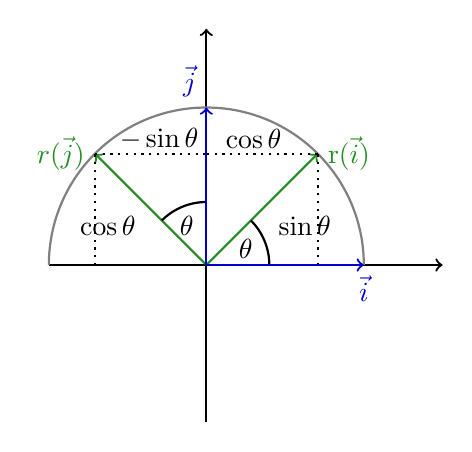
\begin{tikzpicture}

            % Define colors
            \definecolor{greenvec}{RGB}{34,139,34}
            \definecolor{bluevec}{RGB}{0,0,205}
            
            % Draw axes
            \draw[->, thick] (-2,0) -- (3,0); %node[right] {$\hat{e}_x$};
            \draw[->, thick] (0,-2) -- (0,3); %node[above] {$\hat{e}_y$};
            
            % Draw circle (semi-circle)
            \draw[gray, thick] (2,0) arc[start angle=0,end angle=180,radius=2];
            
            % Draw rotated vectors e_x' and e_y'
            \draw[->, thick, greenvec] (0,0) -- ({2*cos(45)},{2*sin(45)}) node[right] {r($\vec{i})$};
            \draw[->, thick, greenvec] (0,0) -- ({-2*sin(45)},{2*cos(45)}) node[left] {$r(\vec{j})$};
            
            % Dotted lines for projections
            \draw[dotted, thick] ({2*cos(45)},0) -- ({2*cos(45)},{2*sin(45)});
            \draw[dotted, thick] ({-2*sin(45)},0) -- ({-2*sin(45)},{2*cos(45)});
            \draw[dotted, thick] ({2*cos(45)},{2*sin(45)}) -- (0,{2*sin(45)});
            \draw[dotted, thick] ({-2*sin(45)},{2*cos(45)}) -- (0,{2*cos(45)});
            
            % Label angles and sin/cos values
            \draw (0.5,0.2) node {$\theta$};
            \draw (.6,1.6) node {$\cos\theta$};
            \draw (1.25,0.5) node {$\sin\theta$};
            \draw (-.6,1.6) node {$-\sin\theta$};
            \draw (-1.25,.5) node {$\cos\theta$};
            \draw (-.25,.5) node {$\theta$};
            
            % Angle arc
            \draw[thick] (0.8,0) arc[start angle=0, end angle=45, radius=0.8];
            \draw[thick] (0,.8) arc[start angle=90, end angle=135, radius=0.8];
            
            % Original basis vectors
            \draw[->, thick, bluevec] (0,0) -- (2,0) node[below] {$\vec{i}$};
            \draw[->, thick, bluevec] (0,0) -- (0,2) node[above left] {$\vec{j}$};
            
            \end{tikzpicture}
        \end{center}

        We could move from here and get more complicated, breaking down each possible vector into sines and cosines and re-interpreting the fundamental right-triangle trigonometry, OR we can make use of linear combinations to do the hard work for us.

        As it turns out, if our original vector $\vec{v}=a\vec{i}+b\vec{j}$, then we can find the rotation of $\vec{v}$ by first rotating $\vec{i}$ and $\vec{j}$, and then using the same scalars $a$ and $b$ to construct the rotated vector $r(\vec{v}) = a \cdot r(\vec{i}) + b \cdot r(\vec{j})$.

        Try it out on a few vectors using the following GeoGebra applet:

        First enter where you want the new basis vectors to go after rotation. For $90^\circ$ rotation, $r(\vec{i})$ should be $\begin{bmatrix} 0 \\ 1 \end{bmatrix}$ and $r(\vec{j})$ should be $\begin{bmatrix} -1 \\ 0 \end{bmatrix}$.

        Then, check the "Track Vector Transformation" box and move the vector $\vec{v}$ to a location of our choosing. Hitting the "Apply Linear Transformation" button will rotate the vector by $90^\circ$, and will display the resulting linear combination of the rotated basis vectors.

        \begin{center}
            \geogebra{uaua5mpa}{1156}{636}
        \end{center}

        Use the applet to find the rotations of the following vectors:

        \begin{enumerate}

            \item $\vec{v}=\begin{bmatrix} 1 \\ 1 \end{bmatrix}$ rotated by $60^\circ$ is (rounded to two decimal places) $\begin{bmatrix} \answer{-.37} \\ \answer{1.37} \end{bmatrix}$.
            
            \item $\vec{v}=\begin{bmatrix} 2 \\ 3 \end{bmatrix}$ rotated by $45^\circ$ is (rounded to two decimal places) $\begin{bmatrix} \answer{-.71} \\ \answer{3.54} \end{bmatrix}$.
            
            \item $\vec{v}=\begin{bmatrix} -1 \\ -2 \end{bmatrix}$ rotated by $30^\circ$ is (rounded to two decimal places) $\begin{bmatrix} \answer{.13} \\ \answer{-2.23} \end{bmatrix}$.
        \end{enumerate}

    \end{example}

    \begin{example}\name{Checking our Work}

        Let's verify that this works for a rotation that we know from the unit circle. If we start at an angle of $\theta = 45^\circ$, the associated vector is 
        
        $$\vec{v}=\begin{bmatrix} \frac{\sqrt{2}}{2} \\ \frac{\sqrt{2}}{2} \end{bmatrix}.$$

        If we rotate by $90^\circ$, we arrive at an angle of $135^\circ$, and the associated vector is 

        $$r(\vec{v}) = \begin{bmatrix} -\frac{\sqrt{2}}{2} \\ \frac{\sqrt{2}}{2} \end{bmatrix}.$$

        If our rotation function $r$ is correct, then we start at $\vec{v}$ so $a=\sqrt{2}/2$ and $b=\sqrt{2}/2$. Then we have for $90^\circ$ rotation, $r(\vec{i})=\begin{bmatrix} 0 \\ 1 \end{bmatrix}$ and $r(\vec{j})=\begin{bmatrix} -1 \\ 0 \end{bmatrix}$, so 

        $$r(\vec{v}) = \frac{\sqrt{2}}{2} \begin{bmatrix} 0 \\ 1 \end{bmatrix} + \frac{\sqrt{2}}{2} \begin{bmatrix} -1 \\ 0 \end{bmatrix} = \begin{bmatrix} -\frac{\sqrt{2}}{2} \\ \frac{\sqrt{2}}{2} \end{bmatrix}.$$

        Double check that this matches the rotation seen in the GeoGebra applet.

    \end{example}

    \begin{remark}

        This process of rotation gives us the foundation for building an entire collection of transformations on vectors (and one of the most important interpretations of matrices): The Linear Transformation.

        Our process of rotating vectors was:

        \begin{enumerate}

            \item Rotate the standard basis vectors.
        
            \item Write the original vector as a linear combination of the standard basis vectors.
            
            \item Use the same scalars to construct the new vector as a linear combination of the rotated basis vectors.
            
        \end{enumerate}

        As it turns out, this process defines a whole class of transformations, where we don't just rotate vectors, but can also stretch, shrink, reflect, shear, and more generally apply any kind of transformation we want, as long as we build it from basis vectors.

    \end{remark}

        \begin{definition}\name{Linear transformation}

            A vector function $T:\R^n\to \R^m$ is called a \textbf{linear
              transformation}%
            \index{linear transformation!on $\R^n$}, or simply \textbf{linear}, if it
            satisfies the following two conditions:
            \begin{enumerate}
            \item $T$ preserves addition, i.e., for all\/
              $\vect{v},\vect{w}\in\R^n$, we have
              $T(\vect{v}+\vect{w}) = T(\vect{v}) + T(\vect{w})$;
            \item $T$ preserves scalar multiplication, i.e, for all\/
              $\vect{v}\in\R^n$ and scalars $k$, we have
              $T(k\vect{v}) = kT(\vect{v})$.
            \end{enumerate}

            Said differently, linear transformations are built from linear combinations of basis vectors.
          \end{definition}

        More importantly, this also gives us a key operation for matrices: matrix-vector multiplication. 

        If we interpret the columns of a matrix $A$ as the transformations of the standard basis vectors, then the product $A\vec{v}$ of $A$ with any vector $\vec{v}$ is the transformed vector of $\vec{v}$. From this, we define matrix-vector multiplcation in the following way:

        \begin{definition}\name{Matrix-Vector Multiplication}

            Let $A$ be an $m\times n$ matrix and $\vec{v}$ be a vector in $\R^n$. The product $A\vec{v}$ is the vector in $\R^m$ obtained from the following operations:
            
            \begin{enumerate}

                \item Form $n$ vectors in $\R^m$ from the columns of $A$, denoted $A\vec{e}_1, A\vec{e}_2, \ldots, A\vec{e}_n$. These are the transformed standard basis vectors of $\R^n$, $\vec{e}_1, \vec{e}_2, \ldots, \vec{e}_n$.
                
                \item Form $n$ scalars $v_1, v_2, \ldots, v_n$ from the entries of $\vec{v}$.
                
                \item Build $A\vec{v}$ as the linear combination of the transformed standard basis vectors:
                
                $$A\vec{v} = v_1A\vec{e}_1 + v_2A\vec{e}_2 + \cdots + v_nA\vec{e}_n.$$

            \end{enumerate}
        \end{definition}

        Unlike scalar multiplication, matrix-vector multiplication requires that the column dimension of the matrix matches the vector dimension, and guarantees that the resulting vector's dimension matches the row dimension of the matrix. This means that matrix-vector multiplication won't always be possible for any pair of matrices and vectors.

        \begin{example}

            Verify that the rotations calculated from the GeoGebra applet are the same as the matrix-vector multiplication of the rotation matrix $R$ with the vectors $\vec{v}$.

            Since the rotation matrix $R$ has columns taken from the rotation function, we can write $R=\left[r(\vec{e}_1), r(\vec{e}_2)\right]=\begin{bmatrix} \cos\theta & -\sin\theta \\ \sin\theta & \cos\theta \end{bmatrix}$.

            Let's first do a quick check with MATLAB, which already has a built-in matrix-vector multiplication using the \texttt{A*v} command. We'll use the rotation matrix $R$ for a $60^\circ$ rotation, and the vector $\vec{v}=\begin{bmatrix} 1 \\ 1 \end{bmatrix}$ from the previous example. 

            Running the code

            \begin{verbatim}
            theta=60;
            R = [cosd(theta) -sind(theta); sind(theta) cosd(theta)];
            v = [1; 1];
            R*v
            \end{verbatim}

            yeilds $\begin{bmatrix} -.37 \\ 1.37 \end{bmatrix}$, which matches the rotation calculated from the GeoGebra applet.

            In the following, write out the rotation matrix $R$, the transformed basis vectors $R\vec{e}_1$ and $R\vec{e}_2$, and the scalars in the linear combination that verify the earlier calculations.

            \begin{enumerate}

                \item For a $45^\circ$ rotation, the rotation matrix $R$ is $\begin{bmatrix} \cos 45 & -\sin 45 \\ \sin 45 & \cos 45 \end{bmatrix} = \begin{bmatrix} \frac{\sqrt{2}}{2} & -\frac{\sqrt{2}}{2} \\ \frac{\sqrt{2}}{2} & \frac{\sqrt{2}}{2} \end{bmatrix}$.
                
                The matrix-vector product $A\vec{v}$, where $\vec{v}=\begin{bmatrix} 2 \\ 3 \end{bmatrix}$, is (use 2 decimal places) $A\vec{v}=\answer{2}\begin{bmatrix} \answer{.71} \\ \answer{.71} \end{bmatrix} + \answer{3}\begin{bmatrix} \answer{-.71} \\ \answer{.71} \end{bmatrix} = \begin{bmatrix} -.71 \\ 3.54 \end{bmatrix}$, just as we calculated earlier.

                \item For a $30^\circ$ rotation, the rotation matrix $R$ is $\begin{bmatrix} \cos 30 & -\sin 30 \\ \sin 30 & \cos 30 \end{bmatrix} = \begin{bmatrix} \frac{\sqrt{3}}{2} & -\frac{1}{2} \\ \frac{1}{2} & \frac{\sqrt{3}}{2} \end{bmatrix}$.
                
                The matrix-vector product $A\vec{v}$, where $\vec{v}=\begin{bmatrix} -1 \\ -2 \end{bmatrix}$, is (use 2 decimal places) $A\vec{v}=\answer{-1}\begin{bmatrix} \answer{.87} \\ \answer{.5} \end{bmatrix} + \answer{-2}\begin{bmatrix} \answer{-.5} \\ \answer{.87} \end{bmatrix} = \begin{bmatrix} .13 \\ -2.23 \end{bmatrix}$, just as we calculated earlier.
            \end{enumerate}

            \begin{hint}
            
                If you want to try out basic rotations from both definitions in a MATLAB file, find the \texttt{mod\textunderscore 2\textunderscore matrix\textunderscore trans.mlx} live script in the course files.

            \end{hint}

        \end{example}



    \begin{example}\name{Rotating the Smile}

        After all of this work, we can finally return to the original problem of rotating the smiley face back to its original orientation.

        All of the smile vectors are $2$-dimensional, so we just need to use a $2\times 2$ rotation matrix to rotate them back. The rotation matrix for a $-90$ degree rotation is $R=\begin{bmatrix} 0 & -1 \\ 1 & 0 \end{bmatrix}$.

        Try it for yourself in the \texttt{mod\textunderscore2\textunderscore matrix\textunderscore trans.mlx} live script. The code is as follows:
        \begin{enumerate}

            \item Load the smiley face with the rotated smile and view the matrices \texttt{face\textunderscore points} and \texttt{smile\textunderscore points}. (Remember that a matrix is an array of vectors, which is how we interpret both of these matrices).
            \begin{verbatim}
            load +linalg/separate_face_points.mat
            face_points
            smile_points
            \end{verbatim}

            \item Re-write each vector (row) $\vec{v}$ in \texttt{smile\textunderscore points} as the rotated vector $R*\vec{v}$, where $R$ is the rotation matrix for a $-90$ degree rotation.
            
            \begin{verbatim}
            theta=-90
            R=[cosd(theta), -sind(theta);
                sind(theta), cosd(theta)]
            for i=1:length(smile_points)
                %NOTE: You need to transpose the vector in smile_points 
                %so that the dimensions match, R is 2x2 and v is 1x2, 
                %so we want v' the 2x1 transpose
                smile_points(i,:)=R*smile_points(i,:)';
            end
            \end{verbatim}

            \item Check that the rotation worked!
            
            \begin{verbatim}
            linalg.plot_img_points(smile_points)
            hold on
            linalg.plot_img_points(face_points)
            hold off
            \end{verbatim}

        \end{enumerate}

        The resulting plot should show the smiley face with the smile back in its original orientation.

    \end{example}

\section*{Other Useful Transformation Matrices}

    While rotations are common, and actually quite important, there are plenty of other useful transformations that are usefl to know. These also give great opportunities to practice writing linear transformations as matrix-vector products!

    You'll go over these in more detail during the discussion activity, but here is an overview of some of the more common transformations.

    \begin{example}\name{Common Transformations}

        We'll now examine other commonly-used linear transformations that have nice properties. These transfromations are useful in computer graphics, physics, and other fields. 

        All of these transformations have $3$-dimensional analogues, but we'll start with the $2$-dimensional versions.

        Remember that the most important information for a linear transformation is how it transforms the standard basis vectors.

        \begin{enumerate}

            \item {\bf Reflection:} Let $T:\R^2\to\R^2$ be a reflection about the $y$-axis. Find the
            matrix%
            \index{matrix!of a reflection}%
            \index{reflection!matrix of}%
            \index{linear transformation!reflection} $A$ corresponding to this
            linear transformation, and a formula for $T$.
          
          \begin{solution}
            The before-and-after picture for a reflection about the $y$-axis
            looks like this:
            \begin{center}
              \begin{tikzpicture}
                \begin{scope}[scale=0.5]
                  \draw[red,thick,fill=red!15]
                  (0,0) -- (0,5) -- (3,5) -- (3,4) -- (1,4) --
                  (1,3) -- (2,3) -- (2,2) -- (1,2) -- (1,0) -- cycle;
                  \draw[step=1cm, gray!50, very thin] (-5.8,-5.8) grid (5.8,5.8);
                  \draw[semithick,->] (-6.5,0) -- (6.5,0);
                  \draw[semithick,->] (0,-6.5) -- (0,6.5);
                  \draw[red,thick]
                  (0,0) -- (0,5) -- (3,5) -- (3,4) -- (1,4) --
                  (1,3) -- (2,3) -- (2,2) -- (1,2) -- (1,0) -- cycle;
                  \draw[blue,thick,->] (0,0) -- node[below] {$\vect{e}_1$} (5,0);
                  \draw[blue,thick,->] (0,0) -- node[left] {$\vect{e}_2$} (0,5);
                \end{scope}
                \begin{scope}[xshift=4.5cm]
                  \path (0,0) node {$\stackrel{T}{\longmapsto}$};
                \end{scope}
                \begin{scope}[xshift=9cm,scale=0.5]
                  \draw[red,thick,fill=red!15,xscale=-1]
                  (0,0) -- (0,5) -- (3,5) -- (3,4) -- (1,4) --
                  (1,3) -- (2,3) -- (2,2) -- (1,2) -- (1,0) -- cycle;
                  \draw[step=1cm, gray!50, very thin] (-5.8,-5.8) grid (5.8,5.8);
                  \draw[semithick,->] (-6.5,0) -- (6.5,0);
                  \draw[semithick,->] (0,-6.5) -- (0,6.5);
                  \draw[red,thick,xscale=-1]
                  (0,0) -- (0,5) -- (3,5) -- (3,4) -- (1,4) --
                  (1,3) -- (2,3) -- (2,2) -- (1,2) -- (1,0) -- cycle;
                  \draw[blue,thick,->,xscale=-1] (0,0) -- node[below]
                  {$T(\vect{e}_1) = \begin{bmatrix}-1\\0\end{bmatrix}$}
                  (5,0);
  \draw[blue,thick,->,xscale=-1] (0,0) --
                  node[right] {$T(\vect{e}_2) = \begin{bmatrix}0\\1\end{bmatrix}$}
                  (0,5);
                \end{scope}
              \end{tikzpicture}
            \end{center}
            We see that
            \begin{equation*}
              T(\vect{e}_1) = -\vect{e}_1 = \begin{bmatrix}-1\\0\end{bmatrix}
              \quad\mbox{and}\quad
              T(\vect{e}_2) = \vect{e}_2 = \begin{bmatrix}0\\1\end{bmatrix}.
            \end{equation*}
            Therefore, the matrix of $T$ is
            \begin{equation*}
              A = \begin{bmatrix}
                -1 & 0 \\
                0  & 1 \\
              \end{bmatrix}.
            \end{equation*}
          \end{solution}

          \item We describe the linear transformation that is given by each of the
            following matrices in terms of reflections, rotations, and scalings:
            \begin{enumerate}
                \item 
            \begin{equation*}
              \quad
              A = \begin{bmatrix}
                0 & 1 \\
                1 & 0 \\
              \end{bmatrix}
            \end{equation*}

            \begin{solution}
                To draw each before-and-after picture, we can start by drawing the
                images of the two standard basis vectors $\vec{e}_1$ and
                $\vec{e}_2$, which are the columns of the transformation matrix. We
                have also drawn the image of the letter ``F'', to better illustrate
                the effect of each transformation.
                \begin{center}
                  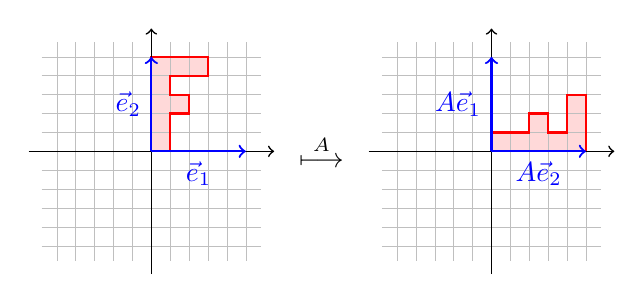
\begin{tikzpicture}[scale=0.96]
                    \begin{scope}

                      \begin{scope}[scale=0.25]
                        \draw[red,thick,fill=red!15]
                        (0,0) -- (0,5) -- (3,5) -- (3,4) -- (1,4) --
                        (1,3) -- (2,3) -- (2,2) -- (1,2) -- (1,0) -- cycle;
                        \draw[step=1cm, gray!50, very thin] (-5.8,-5.8) grid (5.8,5.8);
                        \draw[red,thick]
                        (0,0) -- (0,5) -- (3,5) -- (3,4) -- (1,4) --
                        (1,3) -- (2,3) -- (2,2) -- (1,2) -- (1,0) -- cycle;
                        \draw[semithick,->] (-6.5,0) -- (6.5,0);
                        \draw[semithick,->] (0,-6.5) -- (0,6.5);
                        \draw[blue,thick,->] (0,0) -- node[below] {$\vec{e}_1$} (5,0);
                        \draw[blue,thick,->] (0,0) -- node[left] {$\vec{e}_2$} (0,5);
                      \end{scope}
                      \begin{scope}[xshift=2.25cm]
                        \path (0,0) node {$\stackrel{A}{\longmapsto}$};
                      \end{scope}
                      \begin{scope}[xshift=4.5cm,scale=0.25]
                        \draw[red,thick,fill=red!15,cm={0,1,1,0,(0,0)}]
                        (0,0) -- (0,5) -- (3,5) -- (3,4) -- (1,4) --
                        (1,3) -- (2,3) -- (2,2) -- (1,2) -- (1,0) -- cycle;
                        \draw[step=1cm, gray!50, very thin] (-5.8,-5.8) grid (5.8,5.8);
                        \draw[red,thick,cm={0,1,1,0,(0,0)}]
                        (0,0) -- (0,5) -- (3,5) -- (3,4) -- (1,4) --
                        (1,3) -- (2,3) -- (2,2) -- (1,2) -- (1,0) -- cycle;
                        \draw[semithick,->] (-6.5,0) -- (6.5,0);
                        \draw[semithick,->] (0,-6.5) -- (0,6.5);
                        \draw[blue,thick,->,cm={0,1,1,0,(0,0)}] (0,0) --
                        node[left] {$A\vec{e}_1$} (5,0);
                        \draw[blue,thick,->,cm={0,1,1,0,(0,0)}] (0,0) --
                        node[below] {$A\vec{e}_2$} (0,5);
                      \end{scope}
                    \end{scope}
                \end{tikzpicture}
                \end{center}

                The transformation $A$ is a reflection%
                \index{matrix!of a reflection}%
                \index{reflection!matrix of}%
                \index{linear transformation!reflection} about the line $x=y$. 

                You might also describe the effect as swapping the positions of the standard basis vectors. This kind of transformation will be important in the next chapter. 
            \end{solution}

        \item 
            \begin{equation*}
              \quad
              B = \begin{bmatrix}
                2 & 0 \\
                0 & 2 \\
              \end{bmatrix},\quad
            \end{equation*}

            \begin{solution}
                \begin{center}
                    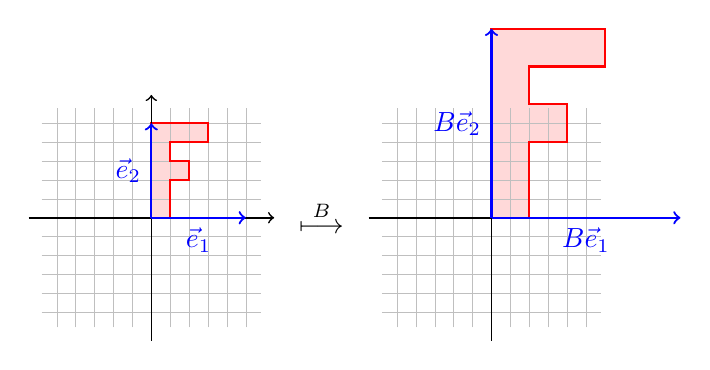
\begin{tikzpicture}[scale=0.96]
                    \begin{scope}[xshift=9cm]
                      \begin{scope}[scale=0.25]
                        \draw[red,thick,fill=red!15]
                        (0,0) -- (0,5) -- (3,5) -- (3,4) -- (1,4) --
                        (1,3) -- (2,3) -- (2,2) -- (1,2) -- (1,0) -- cycle;
                        \draw[step=1cm, gray!50, very thin] (-5.8,-5.8) grid (5.8,5.8);
                        \draw[red,thick]
                        (0,0) -- (0,5) -- (3,5) -- (3,4) -- (1,4) --
                        (1,3) -- (2,3) -- (2,2) -- (1,2) -- (1,0) -- cycle;
                        \draw[semithick,->] (-6.5,0) -- (6.5,0);
                        \draw[semithick,->] (0,-6.5) -- (0,6.5);
                        \draw[blue,thick,->] (0,0) -- node[below] {$\vec{e}_1$} (5,0);
                        \draw[blue,thick,->] (0,0) -- node[left] {$\vec{e}_2$} (0,5);
                      \end{scope}
                      \begin{scope}[xshift=2.25cm]
                        \path (0,0) node {$\stackrel{B}{\longmapsto}$};
                      \end{scope}
                      \begin{scope}[xshift=4.5cm,scale=0.25]
                        \draw[red,thick,fill=red!15,cm={2,0,0,2,(0,0)}]
                        (0,0) -- (0,5) -- (3,5) -- (3,4) -- (1,4) --
                        (1,3) -- (2,3) -- (2,2) -- (1,2) -- (1,0) -- cycle;
                        \draw[step=1cm, gray!50, very thin] (-5.8,-5.8) grid (5.8,5.8);
                        \draw[red,thick,cm={2,0,0,2,(0,0)}]
                        (0,0) -- (0,5) -- (3,5) -- (3,4) -- (1,4) --
                        (1,3) -- (2,3) -- (2,2) -- (1,2) -- (1,0) -- cycle;
                        \draw[semithick] (-6.5,0) -- (6.5,0);
                        \draw[semithick] (0,-6.5) -- (0,6.5);
                        \draw[blue,thick,->,cm={2,0,0,2,(0,0)}] (0,0) --
                        node[below] {$B\vec{e}_1$} (5,0);
                        \draw[blue,thick,->,cm={2,0,0,2,(0,0)}] (0,0) --
                        node[left] {$B\vec{e}_2$} (0,5);
                      \end{scope}
                    \end{scope}
                    \end{tikzpicture}
                \end{center}

                The
                transformation $B$ is a scaling%
                \index{matrix!of a scaling}%
                \index{scaling!matrix of}%
                \index{linear transformation!scaling} by a factor of $2$. 
    
            \end{solution}

        \item 
        \begin{equation*}
            C = \begin{bmatrix}
              \frac{1}{2} & 0 \\
              0 & 2 \\
            \end{bmatrix}
        \end{equation*}

            \begin{solution}
                \begin{center}
                    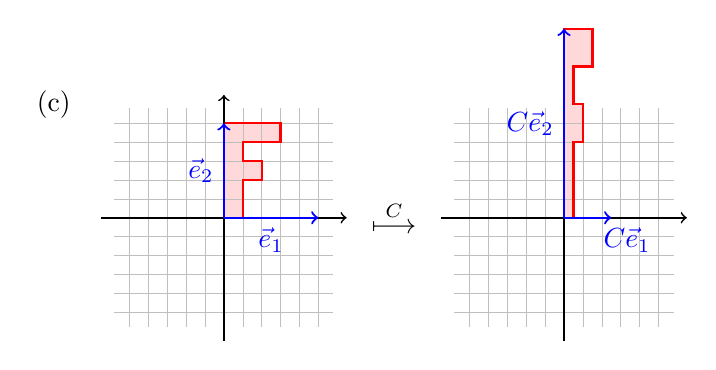
\begin{tikzpicture}[scale=0.96]
                    \begin{scope}[yshift=-3.75cm]
                      \path (-2.25,1.5) node {(c)};
                      \begin{scope}[scale=0.25]
                        \draw[red,thick,fill=red!15]
                        (0,0) -- (0,5) -- (3,5) -- (3,4) -- (1,4) --
                        (1,3) -- (2,3) -- (2,2) -- (1,2) -- (1,0) -- cycle;
                        \draw[step=1cm, gray!50, very thin] (-5.8,-5.8) grid (5.8,5.8);
                        \draw[red,thick]
                        (0,0) -- (0,5) -- (3,5) -- (3,4) -- (1,4) --
                        (1,3) -- (2,3) -- (2,2) -- (1,2) -- (1,0) -- cycle;
                        \draw[semithick,->] (-6.5,0) -- (6.5,0);
                        \draw[semithick,->] (0,-6.5) -- (0,6.5);
                        \draw[blue,thick,->] (0,0) -- node[below] {$\vec{e}_1$} (5,0);
                        \draw[blue,thick,->] (0,0) -- node[left] {$\vec{e}_2$} (0,5);
                      \end{scope}
                      \begin{scope}[xshift=2.25cm]
                        \path (0,0) node {$\stackrel{C}{\longmapsto}$};
                      \end{scope}
                      \begin{scope}[xshift=4.5cm,scale=0.25]
                        \draw[red,thick,fill=red!15,cm={0.5,0,0,2,(0,0)}]
                        (0,0) -- (0,5) -- (3,5) -- (3,4) -- (1,4) --
                        (1,3) -- (2,3) -- (2,2) -- (1,2) -- (1,0) -- cycle;
                        \draw[step=1cm, gray!50, very thin] (-5.8,-5.8) grid (5.8,5.8);
                        \draw[red,thick,cm={0.5,0,0,2,(0,0)}]
                        (0,0) -- (0,5) -- (3,5) -- (3,4) -- (1,4) --
                        (1,3) -- (2,3) -- (2,2) -- (1,2) -- (1,0) -- cycle;
                        \draw[semithick,->] (-6.5,0) -- (6.5,0);
                        \draw[semithick] (0,-6.5) -- (0,6.5);
                        \draw[blue,thick,->,cm={0.5,0,0,2,(0,0)}] (0,0) --
                        node[below,xshift=0.5cm] {$C\vec{e}_1$} (5,0);
                        \draw[blue,thick,->,cm={0.5,0,0,2,(0,0)}] (0,0) --
                        node[left] {$C\vec{e}_2$} (0,5);
                      \end{scope}
                    \end{scope}
                    \end{tikzpicture}
                \end{center}

                The
                transformation $C$ is also a scaling, but by a different factor in
                the $x$- and $y$-directions. It scales the $x$-direction by a factor
                of $\frac{1}{2}$ (or equivalently, shrinks it by a factor of $2$),
                and scales the $y$-direction by a factor of $2$. 

            \end{solution}

            \item 
        \begin{equation*}
              D = \begin{bmatrix}
                1 & 1 \\
                0 & 1 \\
              \end{bmatrix}.
            \end{equation*}
          
        
        \begin{solution}
            \begin{center}
                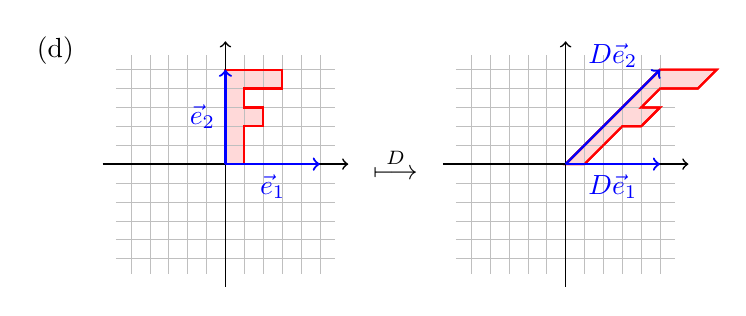
\begin{tikzpicture}[scale=0.96]
                \begin{scope}[xshift=9cm,yshift=-3.75cm]
                  \path (-2.25,1.5) node {(d)};
                  \begin{scope}[scale=0.25]
                    \draw[red,thick,fill=red!15]
                    (0,0) -- (0,5) -- (3,5) -- (3,4) -- (1,4) --
                    (1,3) -- (2,3) -- (2,2) -- (1,2) -- (1,0) -- cycle;
                    \draw[step=1cm, gray!50, very thin] (-5.8,-5.8) grid (5.8,5.8);
                    \draw[red,thick]
                    (0,0) -- (0,5) -- (3,5) -- (3,4) -- (1,4) --
                    (1,3) -- (2,3) -- (2,2) -- (1,2) -- (1,0) -- cycle;
                    \draw[semithick,->] (-6.5,0) -- (6.5,0);
                    \draw[semithick,->] (0,-6.5) -- (0,6.5);
                    \draw[blue,thick,->] (0,0) -- node[below] {$\vec{e}_1$} (5,0);
                    \draw[blue,thick,->] (0,0) -- node[left] {$\vec{e}_2$} (0,5);
                  \end{scope}
                  \begin{scope}[xshift=2.25cm]
                    \path (0,0) node {$\stackrel{D}{\longmapsto}$};
                  \end{scope}
                  \begin{scope}[xshift=4.5cm,scale=0.25]
                    \draw[red,thick,fill=red!15,cm={1,0,1,1,(0,0)}]
                    (0,0) -- (0,5) -- (3,5) -- (3,4) -- (1,4) --
                    (1,3) -- (2,3) -- (2,2) -- (1,2) -- (1,0) -- cycle;
                    \draw[step=1cm, gray!50, very thin] (-5.8,-5.8) grid (5.8,5.8);
                    \draw[red,thick,cm={1,0,1,1,(0,0)}]
                    (0,0) -- (0,5) -- (3,5) -- (3,4) -- (1,4) --
                    (1,3) -- (2,3) -- (2,2) -- (1,2) -- (1,0) -- cycle;
                    \draw[semithick,->] (-6.5,0) -- (6.5,0);
                    \draw[semithick,->] (0,-6.5) -- (0,6.5);
                    \draw[blue,thick,->,cm={1,0,1,1,(0,0)}] (0,0) --
                    node[below] {$D\vec{e}_1$} (5,0);
                    \draw[blue,thick,->,cm={1,0,1,1,(0,0)}] (0,0) --
                    node[above,yshift=0.5cm] {$D\vec{e}_2$} (0,5);
                  \end{scope}
                \end{scope}
              \end{tikzpicture}
            \end{center}

            The transformation
            $D$ is called a \textbf{shearing}%
            \index{matrix!of a shearing}%
            \index{shearing!matrix of}%
            \index{linear transformation!shearing}. It keeps one line (the
            $x$-axis) fixed, while shifting all other points by varying
            distances along lines that are parallel to the $x$-axis.

          \end{solution}
        \end{enumerate}

        

        \end{enumerate}

    \end{example}


\end{document}